%% This is file `elsarticle-template-1-num.tex',
%%
%% Copyright 2009 Elsevier Ltd
%%
%% This file is part of the 'Elsarticle Bundle'.
%% ---------------------------------------------
%%
%% It may be distributed under the conditions of the LaTeX Project Public
%% License, either version 1.2 of this license or (at your option) any
%% later version.  The latest version of this license is in
%%    http://www.latex-project.org/lppl.txt
%% and version 1.2 or later is part of all distributions of LaTeX
%% version 1999/12/01 or later.
%%
%% The list of all files belonging to the 'Elsarticle Bundle' is
%% given in the file `manifest.txt'.
%%
%% Template article for Elsevier's document class `elsarticle'
%% with numbered style bibliographic references
%%
%% $Id: elsarticle-template-1-num.tex 149 2009-10-08 05:01:15Z rishi $
%% $URL: http://lenova.river-valley.com/svn/elsbst/trunk/elsarticle-template-1-num.tex $
%%

%\documentclass[preprint,authoryear,review,12pt]{elsarticle}
\documentclass[preprint,1p,times]{elsarticle}

%% Use the option review to obtain double line spacing
%% \documentclass[preprint,review,12pt]{elsarticle}

%% Use the options 1p,two column; 3p; 3p,twocolumn; 5p; or 5p,twocolumn
%% for a journal layout:
%% \documentclass[final,1p,times]{elsarticle}
%% \documentclass[final,1p,times,twocolumn]{elsarticle}
%% \documentclass[final,3p,times]{elsarticle}
%% \documentclass[final,3p,times,twocolumn]{elsarticle}
%% \documentclass[final,5p,times]{elsarticle}
%% \documentclass[final,5p,times,twocolumn]{elsarticle}


\usepackage{color}
\usepackage{multirow,booktabs,ctable,array}
\usepackage{lscape}
\usepackage{amsmath}
\usepackage{lineno}
\usepackage{ulem}
\usepackage{setspace}
\usepackage{listings}
\usepackage{float}
\usepackage{listings}
\usepackage{color}
\usepackage{rccol}
\usepackage{hyperref}
\usepackage[table]{xcolor}

    \definecolor{listcomment}{rgb}{0.0,0.5,0.0}
    \definecolor{listkeyword}{rgb}{0.0,0.0,0.5}
    \definecolor{listnumbers}{gray}{0.65}
    \definecolor{listlightgray}{gray}{0.955}
    \definecolor{listwhite}{gray}{1.0}

\newcommand{\lstsetcpplong}
{
\lstset{frame = tb,
        framerule = 0.25pt,
        float,
        fontadjust,
        backgroundcolor={\color{listlightgray}},
        basicstyle = {\ttfamily\scriptsize},
        keywordstyle = {\ttfamily\color{listkeyword}\textbf},
        identifierstyle = {\ttfamily},
        commentstyle = {\ttfamily\color{listcomment}\textit},
        stringstyle = {\ttfamily},
        showstringspaces = false,
        showtabs = false,
        numbers = none,
        numbersep = 6pt,
        numberstyle={\ttfamily\color{listnumbers}},
        tabsize = 2,
        language=,
        floatplacement=!h,
        caption={\small \baselineskip 12pt DiReCT long command line menu which is invoked using the `{\ttfamily {-}{-}help}' option.  The short command line menu is obtained by typing `{\ttfamily {-}h}'},
        captionpos=b,
        label=listing:long
        }
}

\floatstyle{plain}
\newfloat{command}{thp}{lop}
\floatname{command}{Command}

%\usepackage[nomarkers,notablist]{endfloat}

%% if you use PostScript figures in your article
%% use the graphics package for simple commands
%% \usepackage{graphics}
%% or use the graphicx package for more complicated commands
%% \usepackage{graphicx}
%% or use the epsfig package if you prefer to use the old commands
%% \usepackage{epsfig}

%% The amssymb package provides various useful mathematical symbols
\usepackage{amssymb}
%% The amsthm package provides extended theorem environments
% \usepackage{amsthm}
 
 \usepackage{makecell}

%% The lineno packages adds line numbers. Start line numbering with
%% \begin{linenumbers}, end it with \end{linenumbers}. Or switch it on
%% for the whole article with \linenumbers after \end{frontmatter}.
%% \usepackage{lineno}

%% natbib.sty is loaded by default. However, natbib options can be
%% provided with \biboptions{...} command. Following options are
%% valid:

%%   round  -  round parentheses are used (default)
%%   square -  square brackets are used   [option]
%%   curly  -  curly braces are used      {option}
%%   angle  -  angle brackets are used    <option>
%%   semicolon  -  multiple citations separated by semi-colon
%%   colon  - same as semicolon, an earlier confusion
%%   comma  -  separated by comma
%%   numbers-  selects numerical citations
%%   super  -  numerical citations as superscripts
%%   sort   -  sorts multiple citations according to order in ref. list
%%   sort&compress   -  like sort, but also compresses numerical citations
%%   compress - compresses without sorting
%%
%% \biboptions{comma,round}

% \biboptions{}

\providecommand{\OO}[1]{\operatorname{O}\bigl(#1\bigr)}

\graphicspath{
             {./Figures/}
             {../SPIE2013/KK/IXI_results/} 
             }

\long\def\symbolfootnote[#1]#2{\begingroup%
\def\thefootnote{\fnsymbol{footnote}}\footnote[#1]{#2}\endgroup}



\journal{NeuroImage}

\begin{document}


\begin{frontmatter}

\title{Functional Image Processing with Advanced Normalization Tools}

\author[label1]{Brian B.~Avants$^\dagger$}
\author[label2]{Nicholas J.~Tustison$^\dagger$
  \fnref{label0}}
  \fntext[label0]{$\dagger$The first two authors contributed equally to this work.}
\author[label1]{Philip A.~Cook}
\author[label1]{Gang Song}
\author[label1]{Jeffrey R.~Duda}
\address[label1]{Penn Image Computing and Science Laboratory, University of Pennsylvania, Philadelphia, PA}
\address[label2]{Department of Radiology and Medical Imaging, University of Virginia, Charlottesville, VA}

\begin{abstract} 
Advanced Normalization Tools (ANTs), combined with R (world's leading
open source statistics software), is appropriate for scanner-to-study
large-scale multiple modality medical image processing.  Here we
summarize a pipeline for using structural T1 imaging data to guide
processing for arterial spin labeling (ASL), resting state functional
MRI (rsfMRI), diffusion tensor MRI (DTI), cortical thickness and
neuroanatomical labeling of major gyri and deep gray matter structures
(thalamus, hippocampi, caudate, putamen, etc.)  We also summarize how
ANTs output may be fed into R to find interpretable statistical models
of population or individual subject data.
\end{abstract}

\begin{keyword}
advanced normalization tools \sep cortical thickness \sep open science
%% keywords here, in the form: keyword \sep keyword
\end{keyword}

\end{frontmatter}
%
%
\newpage
\section{Neuroimaging in Mild TBI}
Traumatic brain injury (TBI) or mild TBI (mTBI) is a risk in both athletics and the
field of duty
\cite{Toblin2012,Peskind2013,Small2013,Kontos2013,Gosselin2012,Zuckerman2012}.
It is identified as the ``signature injury among United States
military personnel involved in combat in Iraq and Afghanistan''
\cite{McCrea2008,Rigg2011}.  
Repeated exposure to mTBI makes recovery increasingly difficult and
leads to long-term susceptibility to recurring injuries
\cite{Shively2012}.  % [NEED BETTER REFERENCE]
mTBI symptoms can be life-altering and
include sleep disturbance \cite{Mysliwiec2013}, difficulties with
working memory \cite{Bryer2013}, increased reaction times
\cite{Luethcke2011}, post-traumatic stress disorder (PTSD)
\cite{Toblin2012,Bazarian2013} and may
lead to long-term psychiatric disorders such as depression
\cite{Mayer2011,Rapp2012,Toblin2012} or a tendency toward newly adopted addictive
behaviors \cite{Miller2013}.  A recent study reveals that up
to 88\% of soldiers returning from combat may have difficulties with sleep
\cite{Mysliwiec2013}.  % search: mild traumatic brain injury soldier
mTBI remains a clinical diagnosis \cite{MacDonald2011} based on self-report measurements
because objective measurements of mTBI remain an active research area \cite{Rapp2012}.
While invasive TBI biomarkers such as PET (requiring injection with a
radioactive isotope) \cite{Small2013} or cerebrospinal fluid
(requiring a spinal tap) have great value \cite{Zetterberg2013}, magnetic resonance imaging
is a powerful and non-invasive instrument that is widely available and captures more direct
information about brain structure/function and the level of injury
\cite{Fox2013}.  Several studies establish advantages of structural
and functional MRI \cite{Ross2013,Yuh2013,Mayer2011,Morey2012}.
T1 MR image processing improves sensitivity for
atrophy detection in mTBI when compared to standard radiological readings \cite{Ross2013}.  Yuh et al \cite{Yuh2013}
estimate that brain imaging doubles the ability to predict cognitive
outcome measurements at three months post-injury.  Diffusion tensor
imaging reveals consistent neuroimaging findings in animals that
relate to repeated exposure to mild TBI and correlate with pathology
\cite{Bennett2012}.  mTBI correlates in DTI are present in veterans
\cite{Morey2012,Jorge2012} and improve longitudinal outcome prediction
at a patient-specific level \cite{Sidaros2008}.  Functional MRI (fMRI) is uniquely able to detect alterations in
both resting and task-adaptive behavior of the brain post-TBI \cite{Roy2010,Mayer2011,Scheibel2012,Stevens2012}.
In summary, multiple MRI modalities are promising biomarkers that 
capture the complex objective sequelae of mTBI that lead to cognitive and behavioral consequences
impairing both quality of life and response to the call of duty.
These objective measurements are therefore valuable in both predicting
outcome and assessing interventional or therapeutic strategies \cite{Roy2010,Rigg2011,Niemeier2011}.
% \cite{MacDonald2013,Huang2013,Bennett2012,Scheibel2012,Simmons2012,Rubovitch2011,MacDonald2011,Risdall2011,Sponheim2011,Roy2010,Maruta2010,DeLellis2009,Rosen2009,Huang2009,Moore2009,Salazar2000}.


\section{Image Processing Methods}

All MRI volumes will be processed using Advanced Normalization Tools
(ANTs) \href{http://www.picsl.upenn.edu/ANTS}{(click here for
link)}\cite{Avants2011a,Avants2011,Murphy2011,Tustison2010,Tustison2011,Tustison2011a}
via previously reported procedures validated as highly accurate
\cite{Klein2009,Klein2010,Murphy2011,Avants2011}.  In general, ANTs-based
processing for multiple modalities is based on, first, defining a
template to guide the population normalization and segmentation
procedures \cite{Avants2011a,Avants2011}.  Traditionally, this
approach was used for single modalities but, more recently, is
exetended for multiple modalities via multiple-modality cohort-specific templates
that capture the average shape and appearance of T1, DTI and
functional images, as in \cite{Kim2010,Avants2011a,Jain2012,Tustison2012}.  We use the
template to guide brain extraction for all modalities and subsequent
tissue or neuroanatomical parcellation \cite{Avants2011a}.  
This general procedure allows several complementary measurements to be
extracted from neuroimaging including 
cortical thickness via DiReCT \cite{Das2009a}, mean diffusion which
may be sensitive to neuronal death, fractional anisotropy,
cerebral blood flow from ASL \cite{Jain2012} or graph connectivity metrics from ASL \cite{Jann2013} or
BOLD \cite{Mayhew2013}.  These measurements, taken together, yield a
multispectral picture of brain health or disease that may have
significant translational value for diagnostics \cite{McMillan2013a} and prognostics \cite{Yuh2013}.

Justification for each modality is described briefly: 

\noindent{\em Jacobian-based Volume from T1-weighted MRI:}  T1 MRI is
typically the highest resolution anatomical image routinely collected
in both clinical and research MRI protocols.  Image registration
methods are able to use T1 MRI to obtain voxel-wise measurement of the
subject structural volume relative to a group local template or
relative to a baseline timepoint.  These measurements are used in
Tensor-Based Morphometry (TBM) which, when performed symmetrically as
in my prior work \cite{Yushkevich2010a,Das2012}, is highly accurate
and provides detailed information on shape change over time
\cite{Brambati2007,Hua2011,Kim2013} or across a population \cite{Kim2008,Massimo2009,Morgan2011,Hanson2010,Hanson2012}.

\noindent{\em Cortical thickness from T1-weighted MRI:}  A measurement that is both sensitive and specific in neurodegeneration \cite{Stricker2012,Libon2012,McMillan2013} and which is associated with cognitive decline \cite{Dickerson2011,Avants2010}.  Quantitative cortical measures have been demonstrated in conditional 
abnormalities such as 
Huntington's disease \citep{rosas2002,rosas2005,selemon2004}, bipolar disorder \cite{lyoo2006}, Alzheimer's disease and frontotemporal
dementia \citep{du2007,dickerson2009}, Parkinson's disease \citep{jubault2011}, Williams syndrome \cite{thompson2005},
multiple sclerosis \citep{ramasamy2009}, autism \citep{chung2005,hardan2006},
migraines \citep{dasilva2007}, chronic smoking \citep{kuhn2010}, alcoholism \citep{fortier2011},
cocaine addiction \citep{makris2008}, Tourette syndrome in children \citep{sowell2008},
scoliosis in
female adolescents \citep{wang2012}, obsessive compulsive
disorder \citep{shin2007}, obesity \citep{raji2010}, and heritable \citep{peterson2009}
and elderly \citep{ballmaier2004} depression.  Cortical thickness also
varies normally as a function of age \citep{kochunov2011},
gender \citep{luders2006a}, untreated transsexuality \citep{zubiaurre-elorza2012},  handedness
\citep{luders2006,amunts2007}, intelligence \citep{shaw2006}, athletic
ability \citep{wei2011}, musical ability \citep{bermudez2009,foster2010}, 
tendency toward criminality \citep{raine2011}, and Tetris-playing
ability in female adolescents \citep{haier2009}. 

\noindent{\em Measurements derived from DTI:}  Fractional anisotropy
measurement of white matter integrity that may reveal the connectivity
components of neurodegeneration \cite{Zhang2009}, aging
\cite{Kochunov2011} potentially captures
a different aspect of the disease process \cite{Englund2004} and may
differentiate tau and TDP-43 effects \cite{McMillan2013b}.  Relatedly,
mean, radial or axial diffusion relate to age and cognition \cite{Wu2011,Pal2011,Bava2011,ODwyer2012,Bjoernebekk2012}, neurodegeneration \cite{Salami2012,Whitwell2010}
and are particularly sensitive to TBI \cite{Huang2009,Fox2013}.

\noindent{\em BOLD or ASL Network Analysis:} BOLD-based network analysis
\cite{Spoormaker2010,Sanz-Arigita2010} has emerged as a powerful tool
with specific value in both brain injury
\cite{Mayer2011,Scheibel2012,Zhou2013}, the study of intervention
strategies \cite{Roy2010,FeldsteinEwing2011} and measurement of pain
\cite{Mayhew2013}.  ASL may also be employed in this manner
\cite{Jann2013} and has been processed with ANTs tools and canonical
correlation analysis \cite{Duda2013}.

\noindent{\em Cerebral blood flow (CBF) from ASL:}  This functional
quantitative measure (versus the relative values provided by BOLD) has
the potential to reveal alterations in the brain due to injury
\cite{Kim2008}, pain \cite{Howard2011}, pharmacological intervention \cite{Black2010,Jenkins2012} or that precede visible structural change and may
indicate cortical reorganization \cite{Hayward2010}.  ASL-based CBF
also accurately recapitulates PET imaging in Alzheimer's disease \cite{Chen2011,Mak2012}.
CBF is a more repeatable functional measurement than BOLD
\cite{Liu2007,Aguirre2012}, may be used in network analysis in lieu of
or combination with 
BOLD \cite{Duda2013} and provides a unique view on the brain complementary to DTI and T1.  

We now detail both general processing strategies and those that are
specific to each modality.

\subsection{ANTs volumetric-based cortical thickness estimation pipeline}

The ANTs-based cortical thickness estimation workflow is illustrated 
in Figure \ref{fig:pipeline}.  The steps are as follows:
\begin{enumerate}
  \item initial N4 bias correction on input anatomical MRI,
  \item brain extraction using a hybrid segmentation/template-based strategy,
  \item alternation between prior-based segmentation and white matter posterior
        probability weighted bias correction,
  \item DiReCT-based cortical thickness estimation, and
  \item optional normalization to specified template.
\end{enumerate}
Each component, including both software and data, is briefly detailed 
below with the relevant references for additional information. 
\begin{figure*}
  \centering
  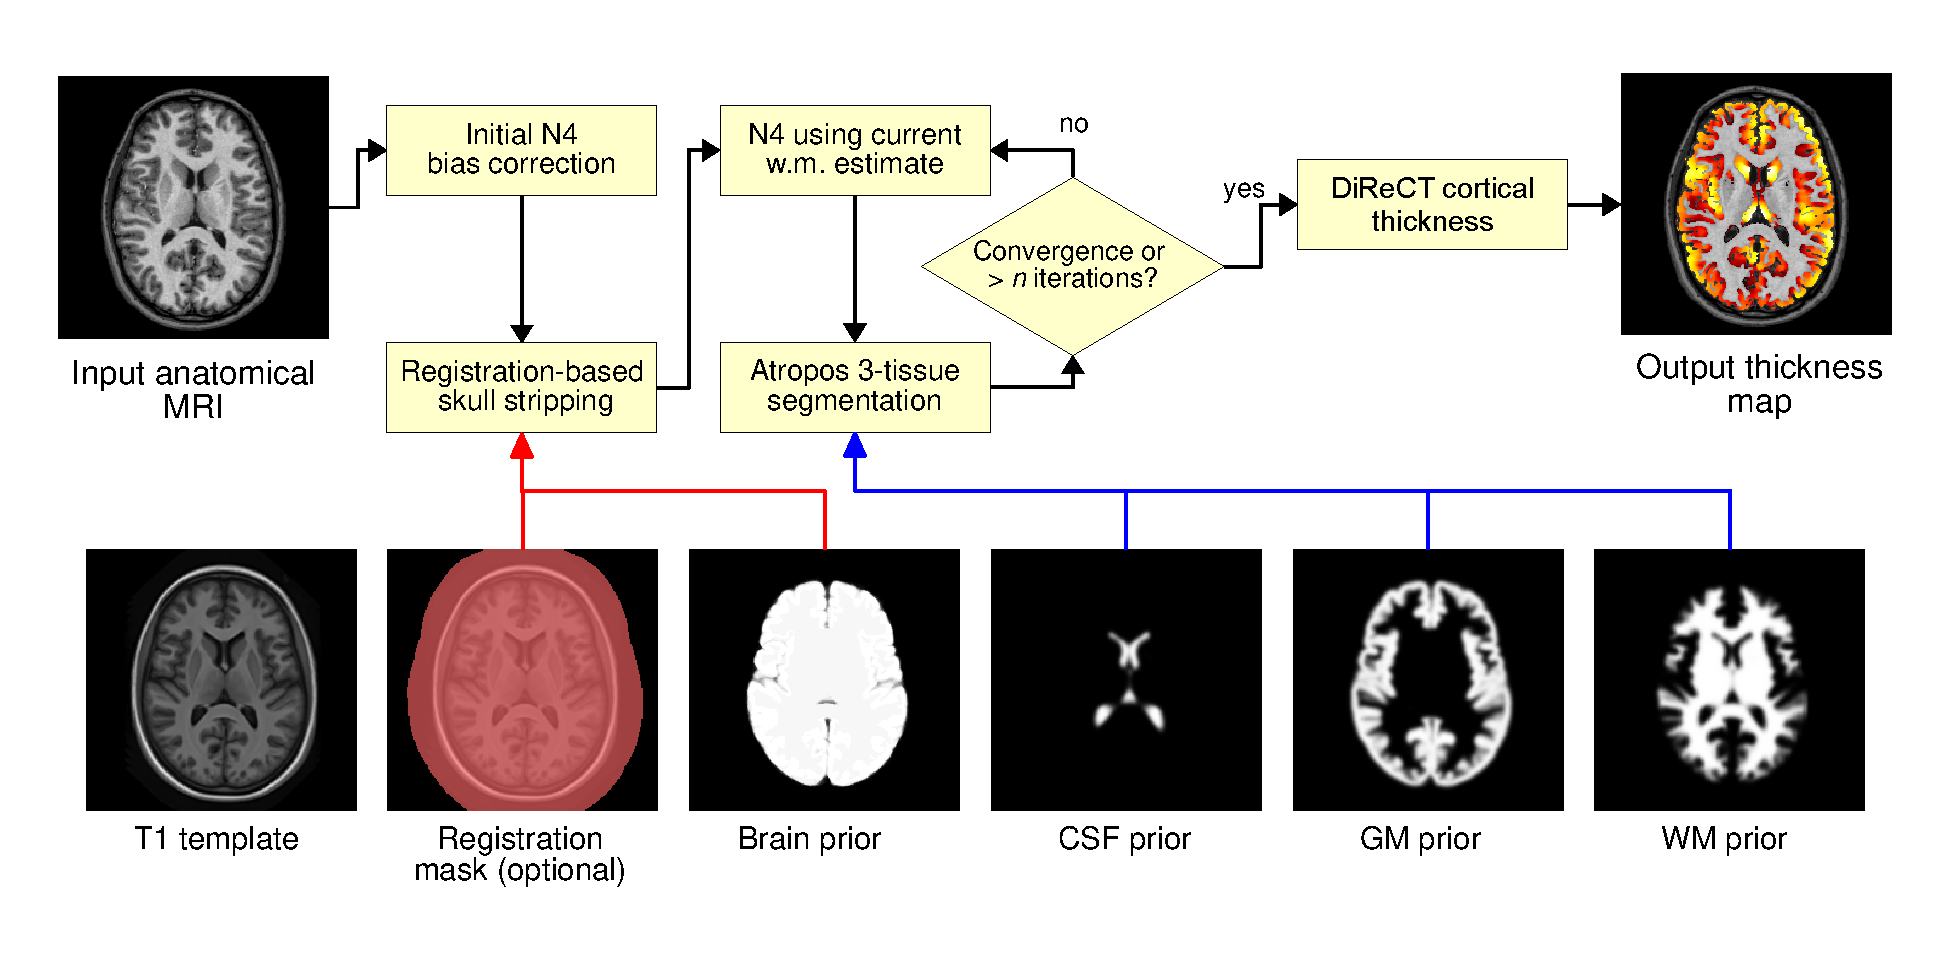
\includegraphics[width=0.9\textwidth]{figs/Kapowski_pipeline2.pdf}
  \caption{Illustration of the main components of the ANTs processing 
  workflow containing all elements for determining cortical thickness. 
  Not shown is the optional subject to template registration.}
  \label{fig:pipeline}
\end{figure*}

\subsubsection{Anatomical template construction}
Normalizing images to a standard coordinate system
reduces intersubject variability in population studies.  Various
approaches exist for determining the normalized space such as the selection
of a pre-existing template based on a single subject, e.g. the Talairach
atlas \citep{Talairach1988}, or a publicly available averaged group of
subjects, e.g. the MNI \citep{Collins1994} or ICBM \citep{Mazziotta1995}
templates.  Additionally, mean templates constructed from labeled
data can be used to construct spatial priors for improving segmentation
algorithms.
The work of \cite{Avants2010} explicitly models the geometric component of the 
normalized space during optimization to produce such mean templates.  Coupling the intrinsic symmetry of 
SyN pairwise registration \citep{Avants2011} and an
optimized shape-based sharpening/averaging of the template appearance, Symmetric Group
Normalization (SyGN) is a powerful framework for producing optimal population-specific
templates \citep{Avants2010}.

\subsubsection{N4 Bias field correction}

Critical to quantitative processing of MRI is the minimization of
field inhomogeneity effects which causes artificial low frequency 
intensity variation across the image.  Large-scale studies, such
as the Alzheimer's Disease Neuroimaging Initiative (ADNI), employ
perhaps the most widely used bias correction algorithm, N3 \cite{sled1998}, 
as part of their standard protocol \citep{boyes2008}.

In \cite{Tustison2010}, we introduced an improvement of N3, denoted as
``N4'', which demonstrates a significant increase in performance and convergence behavior
on a variety of data.  This improvement is a result of an enhanced 
fitting routine (which includes multi-resolution capabilities) and a modified optimization 
formulation.  For our workflow, the additional possibility of specifying
a weighted mask in N4 permits the use of a ``pure tissue'' probability map 
(described below)
calculated during the segmentation pipeline for further improvement of 
bias field estimation.  In addition to its public availability 
through ANTs and the Insight Toolkit, it has also been included in
the popular open source Slicer software package for visualization and medical
image computing \cite{fedorov2011}.

N4 is used in two places during the individual subject processing (cf. Figure
\ref{fig:pipeline}).  Following conversion of the raw dicom T1-weighted image
to Nifti format using our related \verb#Neuropipedream# set of raw image conversion
and organization tools%
\footnote{
http://sourceforge.net/projects/neuropipedream/
}, N4 is used to generate an initial bias corrected image for use in
brain extraction.  The input mask is created by adaptively thresholding 
the background from the foreground using Otsu's algorithm \cite{otsu1979}.
Following brain extraction, three-tissue segmentation involves iterating
between bias field correction using the current pure tissue 
probability map as a weight mask and then using that bias corrected image
as input to the Atropos segmentation step (described in the next section). 

\subsubsection{Atropos 3-tissue segmentation}

In \cite{Avants2011a} we presented an open source $n$-tissue segmentation software tool
(which we denote as ``Atropos'') attempting to distill 20+ years of active research in this area
particularly some of its most seminal work (e.g. \cite{zhang2001,ashburner2005}). 
Specification of prior probabilities includes spatially varying Markov Random Field modeling, 
prior label maps, and prior probability maps typically derived from our template building 
process.  Additional
capabilities include handling of multivariate data, 
partial volume modeling \cite{shattuck2001}, a memory-minimization mode,
label propagation, a plug-n-play architecture for incorporation of novel likelihood models
which includes both parametric and non-parametric models for both scalar and tensorial
images, and alternative posterior formulations for different segmentation tasks.

Due to the important interplay between segmentation and bias correction,
we perform multiple N4 $\Leftrightarrow$ Atropos iterations.
In order to better integrate Atropos and N4, we use  
a pure tissue probability weight mask generated from the 
posterior probabilities generated from the segmentation 
process.  Given $N$ labels and the corresponding $N$
posterior probability maps $\{ P_1, \ldots, P_N\}$ produced
during the segmentation process, the N4 weight mask is 
created at each N4 $\Leftrightarrow$ Atropos iteration from
\begin{align}
  P_{pure\,\,tissue}(\mathbf{x}) = \sum_{i=1}^N P_i(\mathbf{x}) \prod_{j=1, j \neq i}^N \left( 1 - P_j(\mathbf{x}) \right).
\end{align}
One of the key insights of the original N3 algorithm is the
observation that inhomogeneities cause the intensity values of
pure tissue peaks to spread in the intensity histogram as though
convolved with a Gaussian.  A core contribution of N3 is the
proposed corrective of deconvolving the intensity histogram to 
accentuate the tissue peaks coupled with a spatial smoothing 
constraint. The pure tissue probability mask
weights more heavily the voxels corresponding to pure tissue 
types (as determined by the segmentation) during the deconvolution process 
while minimizing the contribution of regions such as the gray/white matter 
interface where peak membership is ambiguous. 

\subsubsection{Brain extraction}

Brain extraction using ANTs combines template building, high-performance
brain image registration \citep{Avants2011}, and Atropos with topological refinements.  
An optimal template for brain extraction is 
generated offline using labeled brain data.  For example, we may use the LPBA40 data \cite{Klein2010}
for generating a brain extraction template and a corresponding brain
probability mask.  In this stage, we use a coarse and relatively fast
registration to calculate a warp between the template whole-head image
and the subject of interest.  The warped template probability map is
thresholded at 0.5 and the resulting mask is dilated with a radius of 2.  Atropos is used to generate an initial 3-tissue segmentation estimate within the mask
region.  Each of the three tissue masks undergo specific morphological operations which are then
combined to create a brain extraction mask for use in the rest of the
cortical thickness workflow. 

A comparison using open access brain data with publicly available
brain extraction algorithms including AFNI's \verb#3dIntracranial#
\citep{ward1999}, FSL's \verb#BET2# \citep{smith2002}, Freesurfer's
\verb#mri_watershed# \citep{segonne2004}, and BrainSuite
\citep{dogdas2005} demonstrated that our combined
registration/segmentation approach \citep{Avants2010a} performs at the
top level alongside BrainSuite (tuned) and FreeSurfer.

\subsubsection{Template-based Morphometry}
We map the brain extracted anatomical image to the group template
brain image using modality-appropriate strategies.  This final high-resolution mapping
to a common coordinate system enables standard voxel-based or
tensor-based morphometry where the Jacobian (or log-Jacobian) derives
from the deformation gradient of the composite mapping between the
individual and the group template brain.  Furthermore, this enables
standardized coordinates to be reported for our multi-modality
statistical analyses (described in section~\ref{sec:R}. 

\subsubsection{DiReCT (aka KellySlater/KellyKapowski) Cortical Thickness Estimation}

DiReCT was introduced 
in \cite{das2009} and made available in ANTs with the program \verb#KellySlater#.
Since then several improvements have been made and incorporated into the program
\verb#KellyKapowski#.  Among the most significant advancements is that the more recent
implementation is multi-threaded, written in rigorous ITK coding style, and 
has been made publicly available through  ANTs complete with a unique user 
interface design developed specifically for ANTs tools.  


\subsubsection{Multi-atlas Anatomical Labeling with ANTs}

Cortical label propagation to each individual subject for all data
sets described below is performed using the PICSL multi-atlas joint
label fusion algorithm described in \cite{wang2013} which recently led
an international competition in multi-atlas segmentation at the MICCAI
2012 Grand Challenge on Multi-Atlas Labeling.  The implementation is
distributed with the ANTs toolkit (program {\em jointfusion}).  Valid
input may include any public population data with anatomical labeling,
e.g. the Nonrigid Image Registration Evaluation Project (NIREP)
label set \citep{christensen2006}.
The initial data set introduced into the project consists of 
16 (8 male and 8 female) high resolution skull-stripped brain 
data with 32 cortical labels (cf. Table \ref{table:nirep_labels}) manually drawn using a 
published protocol.

%Given the gray matter labels, the white matter and CSF were identified 
%for each of the 16 subjects using Atropos.  Similar to the LPBA40
%data set, a NIREP template was created from all 16 subjects and each of the
%warped labels were used to create probabilistic estimates of the 
%labeled region boundaries. These probability maps were used as 
%spatial prior probabilities during the 3-tissue segmentation component
%of the pipeline.  Using SyN, the NIREP template is registered to the
%extracted individual subject brain which is followed by a warping of the 
%NIREP priors to the space of the individual subject.  The initial warped 
%white matter probability map is used as the weighted confidence mask 
%in the follow-up bias correction step.

\begin{table}
\centering
\begin{tabular*}{0.475\textwidth}{@{\extracolsep{\fill}} l l}
\toprule
  1) L occipital lobe & 2) R occipital lobe \\
  3) L cingulate gyrus & 4) R cingulate gyrus \\
  5) L insula gyrus & 6) R insula gyrus \\
  7) L temporal lobe & 8) R temporal lobe \\
  9) L superior temporal gyr. & 10) R superior temporal gyr. \\
  11) L infero temporal region & 12) R infero temporal region \\
  13) L parahippocampal gyr. & 14) R parahippocampal gyr. \\
  15) L frontal pole & 16) R frontal pole \\
  17) L superior frontal gyrus & 18) R superior frontal gyrus \\
  19) L middle frontal gyrus & 20) R middle frontal gyrus \\
  21) L inferior gyrus & 22) R inferior gyrus \\
  23) L orbital frontal gyrus & 24) R orbital frontal gyrus \\
  25) L precentral gyrus & 26) R precentral gyrus \\
  27) L superior parietal lobule & 28) R superior parietal lobule \\
  29) L inferior parietal lobule & 30) R inferior parietal lobule \\
  31) L postcentral gyrus & 32)   R postcentral gyrus \\  
\bottomrule
\end{tabular*}
\caption{The 32 cortical NIREP labels.}
\label{table:nirep_labels}
\end{table}



\subsubsection{DTI Processing with ANTs} 

%Phil --- see
%\href{www.ncbi.nlm.nih.gov/pubmed/23151955‎}{www.ncbi.nlm.nih.gov/pubmed/23151955}
% for content.
Diffusion MRI data consists of a series of images, one or more unweighted images (with no diffusion weighting) and multiple diffusion-weighted images (DWI) sensitized to diffusion along unique directions. The data from all of the images is used to fit a Gaussian model of diffusion in three dimensions, parameterized by the diffusion tensor (DT). The DT encodes complimentary information on the scale, anisotropy, and orientation of apparent diffusion in each voxel, which are sensitive to different aspects of the tissue microstructure, particularly white matter integrity and the local alignment of axon fiber bundles, which we can use to study global white matter connectivity. 

Because of the relatively long imaging time and use of strong gradients, diffusion data is particularly sensitive to misalignment caused by distortion and subject motion. Co-registration of the image volumes is challenging because of limited spatial resolution and highly variable signal to noise ratio in the DWI. After pre-processing and diffusion tensor calculation, we must spatially normalize the diffusion tensors to template space for analysis. We accomplish this by first aligning the diffusion image with the subject's high-resolution T1-weighted image, correcting for any head motion and distortion introduced by differences in the MRI protocols between the T1-weighted image and the DWI. We then combine this intra-subject transformation with the transformation mapping the T1-weighted image to the template space. 

We have developed an automated processing pipeline for diffusion imaging using the open source tools Camino \cite{Cook2006} and ANTs, which provides pre-processing, brain extraction, diffusion tensor computation, and normalization to template space, as well as diagnostic images in the subject space to aid quality control, including fractional anisotropy, average corrected DWI, and noise variance.

The first unweighted image in the diffusion sequence is used as the reference image for motion and distortion correction. The remaining unweighted images are rigidly aligned to the reference image and averaged; this average image is used as the reference image for affine correction of the diffusion-weighted images (DWI) for motion and distortion caused by the diffusion weighting gradients. A brain mask is computed by aligning the average DWI to a template, and warping the template brain mask into the subject space. Processing then continues on the brain-extracted image. Diffusion tensors are calculated using an iterative weighted linear least squares algorithm \cite{Salvador2005}.

Each T1-weighted image is segmented into gray matter, white matter and CSF using N4 bias correction \cite{Tustison2010} and Atropos segmentation \cite{Avants2011a}. The white matter is used as a registration mask for alignment with the corresponding average DWI image. The DWI image is registered to the T1-weighted image using a transform composition derived by optimizing an initial rigid transformation followed by an optimized deformable (symmetric diffeomorphic using SyN \cite{Avants2011}) transform. The rigid transform is found by optimizing the alignment between the average DWI and the masked white matter T1-weighted image of the same subject, to account for motion. The resulting rigid transform is used to initialize distortion correction using the deformable transform.

The transformed DTI are warped to the template space by combining the intra-subject DWI to T1 warp with the warp previously defined to normalize the subject's T1 image to the template space. The correct anatomical orientation of the diffusion tensors is preserved by applying the preservation of principal direction method \cite{Alexander2001}, and scalar statistics such as FA and mean diffusivity are computed from the normalized diffusion tensors.


\subsubsection{Functional Image Processing}

Motion correction is performed by the 
antsMotionCorr program in ANTs which uses a mutual information similarity metric and
a nonlinear conjugate gradient optimizer to maximize the Affine or
Rigid similarity between each image in a time series and a sequence specific reference
image. The reference image for each modality is: BOLD---the average image from the full time
series; CASL and pCASL---the average control labeled image; PASL---the
acquired M0 image.  A brain mask is computed by aligning the reference
motion correction image to a sequence-specific 
template and warping the template brain mask into the subject
space. For ASL-based images, the difference between the tagged and
untagged BOLD signal at each time point is calculated using sinc
subtraction \cite{Liu2005}.  Subsequently, CBF is
quantified using the appropriate acquisition parameters and the
methods of Wang, et al. \cite{Wang2003}. A mean CBF image is created by
averaging over the CBF time-signal. Depending upon processing needs, functional images are
mapped to the T1 individual brain.  Mapping to a group template may
then occur through previously computed coordinate transformations.

Network analysis may be performed with any of three types of input
time series data:  standard BOLD, ASL-BOLD or ASL-CBF.  The ASL-CBF
signal may have advantages over BOLD particularly in the orbitofronal
and anterior temporal regions where standard BOLD signal dropout
occurs \cite{Jann2013,Orosz2012}.  For each time series type we perform:
\newline
\noindent{\em Graph construction:} Cortical labels such as the Automated Anatomical
Labeling (AAL) atlas \cite{Tzourio-Mazoyer2002} are mapped from
the template space into the subject space via the same method used to
generate subject space brain masks described above. For each cortical
and subcortical label, a region-averaged time-signal is
calculated. Each time-series is then bandpass filtered using the
Christiano-Fitzgerald filtering \cite{Christiano2003}, as
implemented by the R function cffilter in package mFilter, to examine
a range of frequencies appropriate for the specific data type. An N$\times$N
correlation matrix is then calculated by finding the correlation
between the filtered time-signals for each of the N labeled regions.
Recent work based on ANTs tools for canonical correlation analysis (CCA) \cite{Avants2010b}
shows that CCA may improve network reliability in both ASL and BOLD
network analysis \cite{Duda2013} and this approach may also be employed.
\newline
\noindent{\em Graph analysis:} To each correlation matrix, sparsity thresholds are
applied to binarize the edges, such that the bottom 50\% to 97.5\% of
the edges are discarded and the remaining edges set to a common
weight of 1.  This approach maintains graph density across subjects
and controls for inter-subject variation in base correlation levels
\cite{Liu2008, Power2011, Schwarz2011, Braun2012, Liang2012}. 
On the binarized graphs, a variety of network measures may be
computed including metrics such as: transitivity,
modularity, efficiency, clustering coefficient, characteristic path
length, and small-worldness. These metrics measure efficiency of
information transmission and community structure, and are calculated
with the R package brainwaver \cite{Achard2006}.


\begin{figure}
  \centering
  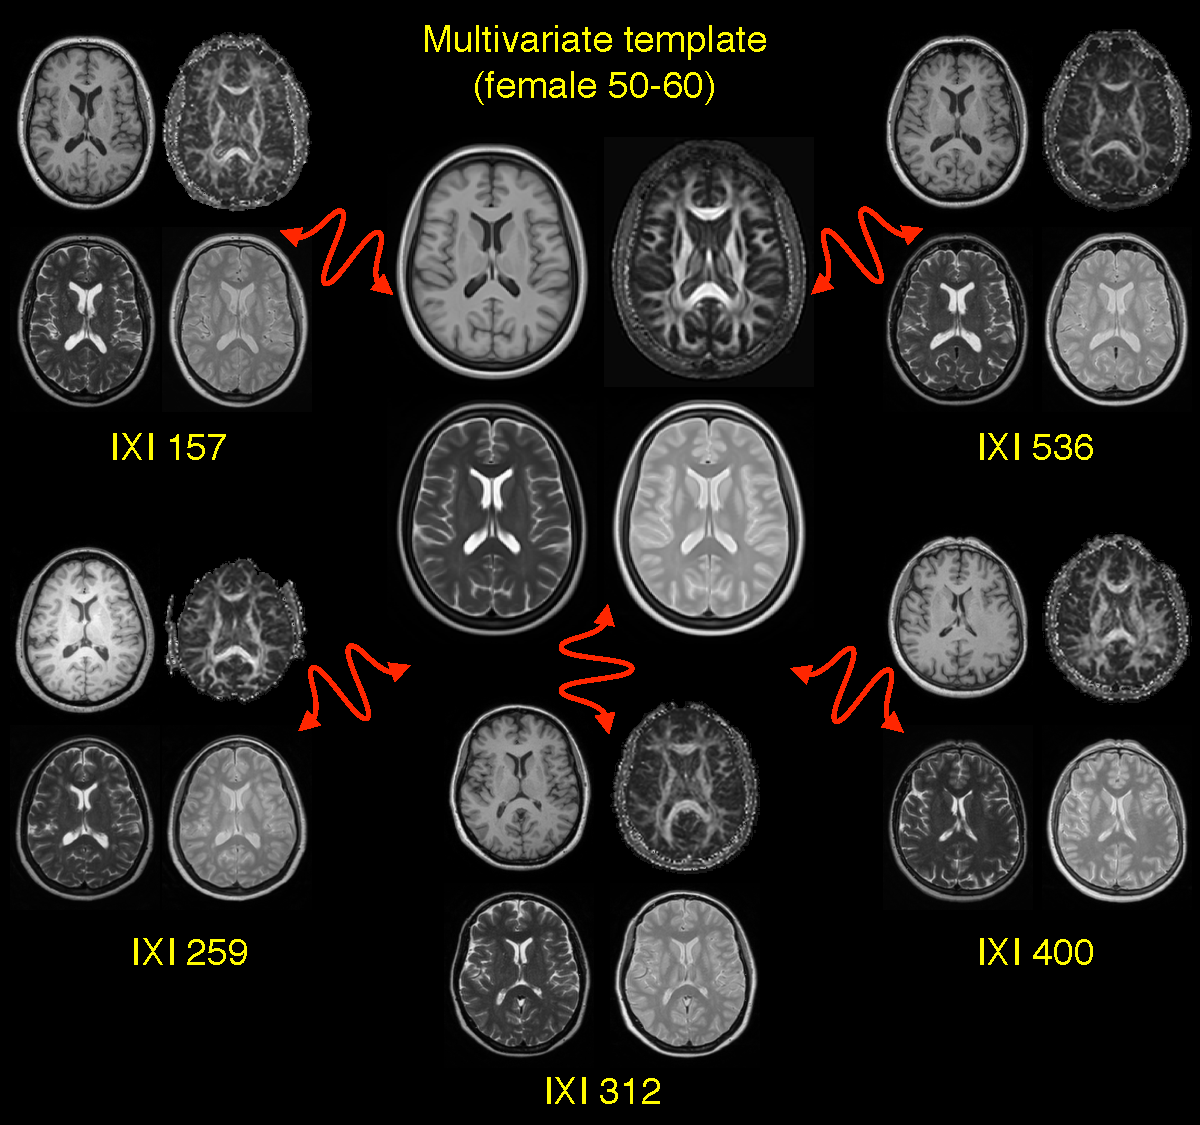
\includegraphics[width=0.8\textwidth]{figs/template50_60.pdf}
  \caption{Sample multivariate template constructed from a subset of the IXI data (female, age 50--60).  Axial slices of five of the 37 total subjects from this cohort are shown. }
  \label{fig:template}
\end{figure}




\section{Statistical Methods}\label{sec:R}
{\small\noindent{\em The first 3 rules of statistics: 'Draw a picture, Draw a picture, Draw a picture.'---Michael Starbird.}  }


R~is a popular
programming/scripting language that is designed to make advanced
statistical analysis accessible.  Because of its ease of use, large user base, and
extensive community development, it is increasingly used by
researchers, statisticians, and data analysts from fields as varied as
economics, machine learning, pharmaceuticals, and finance.  The yearly
useR! conference boasts a sponsor list that includes such diverse
companies as Google, American Credit Acceptance, and the American
Statistical Association.  Virtually all of the most
influential and popular statistical and machine learning algorithms,
including Boosting, the LASSO, and random forests, have associated R
packages, often written by the inventors of the algorithms.  Although
it is difficult to obtain an exact number of R~users, a New York Times
article from 2009 estimated that there are at least 250,000 active R
users, with the number rising each year.  The RStudio company
develops a variety of software technologies, including an integrated
development environment (IDE) and server-side support for running R
programs remotely, that combine to make R~a painless and appealing
programming environment.  Finally, an increasing number of industrial actors, including
Oracle and Revolution Analytics, have begun offering support for R,
helping it gain industrial users.  R~therefore encompasses all the
necessary statistical models for morphometry, linear mixed effects
modeling and machine learning---supplemented with ANTs, we also gain
the necessary image processing core.


\begin{figure}{t}
\begin{center}
  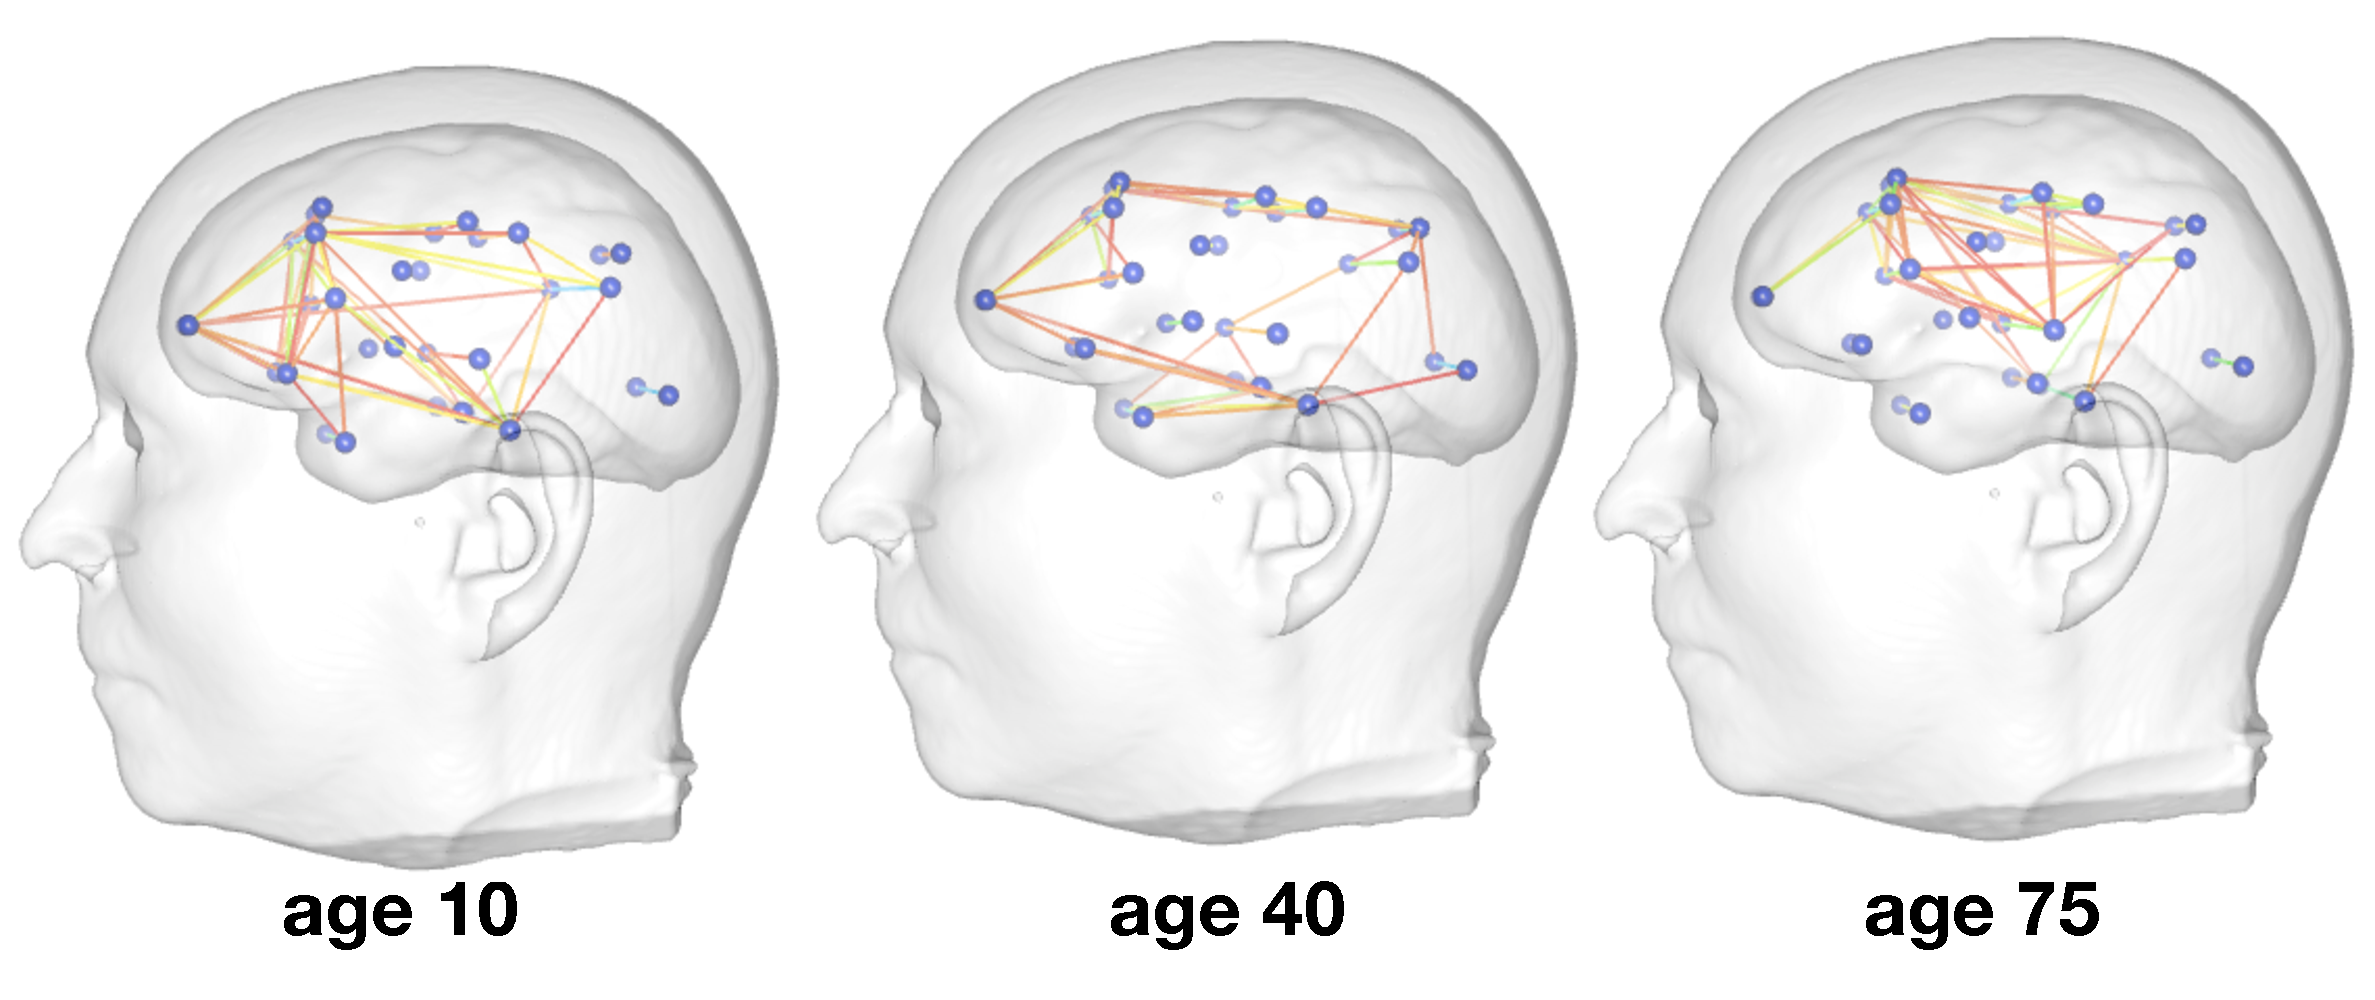
\includegraphics[width=0.9\textwidth]{figs/connx_age}
\end{center}
\caption{ANTsR connectivity analysis shows significant aging effects
  across structural brain networks (n=1200, from public IXI, OASIS, NKI datasets).}\label{fig:cnx}
\end{figure}

When combined with the image processing utilities available in ANTs, R provides a convenient and powerful interface for performing common statistical analyses of imaging data.  In addition, R's standardized syntax minimizes the learning curve for performing a wide variety of different analyses.  The basic form of a statistical model in R is 
\begin{equation}
\text{Outcome} \approx \text{Predictor 1} + \text{Predictor 2} + \text{Predictor 3} + ...
\label{eqn:r_syntax}
\end{equation}
Factor and continuous variable predictors can be combined seamlessly, and a wide variety of model types, including linear models with Gaussian noise, logistic, and Poisson models are available.  When performing a region-of-interest (ROI)-based analysis of the relationship between imaging data and cognition, one typically averages the voxel values within a given ROI and then tests the averaged values against a predictor.  In R syntax, this is written as 
\begin{equation}
\text{ROI value} \approx \text{cognition} + \text{nuisance demographic variables}. 
\label{eqn:ROI}
\end{equation}
Given R's unified interface, conducting voxel-wise morphometric studies of cortical thickness or fractional anisotropy (FA) are similarly easy, with the only difference from Equation \ref{eqn:ROI} being that instead of the ROI value, the original voxel thickness or FA values are provided.  

ANTsR also enables more sophisticated functional studies.  ANTs provides utilities for all necessary preprocessing of time-series data, including motion correction, detrending, and noise reduction (CompCor).  Due to the ease of using factorial predictors in R, task-based fMRI images can be described using the same syntax: 
\begin{equation}
\text{Preprocessed fMRI data} \approx \text{Presence of task} + \text{nuisance regressors}.
\label{eqn:fmri}
\end{equation}
The flexibility of R's linear model functionality also makes tasks that are not typically thought of as regression problems easy to perform.  For example, partial volume corrections in cerebral blood flow (CBF) measurements are often performed using correction equations that can be written as a linear model: 
\begin{equation}
\text{CBF} \approx \text{Percent gray matter} + \text{Percent white matter} + \text{Percent CSF}
\end{equation}
Taking the residual of this model (i.e., the portion of CBF that is not explained by the tissue distribution within a given voxel) is equivalent to performing a partial volume correction.  Once corrected for partial volume effect, the data can be processed using the same method as Equation \ref{eqn:fmri}. 


\section*{Acknowledgments}

\section*{References}

\bibliographystyle{elsarticle-harv}
\bibliography{src/references}


%% Authors are advised to submit their bibtex database files. They are
%% requested to list a bibtex style file in the manuscript if they do
%% not want to use model1-num-names.bst.

%% References without bibTeX database:

% \begin{thebibliography}{00}

%% \bibitem must have the following form:
%%   \bibitem{key}...
%%

% \bibitem{}

% \end{thebibliography}


\end{document}

%%
%% End of file `elsarticle-template-1-num.tex'.
